\chapter{Backstepping}
Este es un método para construir una \gls{flc} para una clase especial de sistemas.\\

\rmk{
	También se puede encontrar en la literatura el \textit{Forwarding}, pero no se aborda debido a que es, en general, un método más complicado.
}
\section{El caso más simple: Backstepping de integrador}
La idea básica del método conocido como \textbf{backstepping} es la siguiente se puede expñlicar, en su forma más simple, considerando el sistema con entrada escalar
\begin{equation}
	\begin{aligned}
		\dot{\eta} & = f(\eta) + g(\eta)\xi                                    \\
		\dot{\xi}  & = u, \quad \eta \in \mathbb{R}, \quad \xi \in \mathbb{R}.
	\end{aligned}
	\label{eq: backstepping_integrador}
\end{equation}
Nótese que este sistema se puede ver como una conexión en cascada, donde el maestro es un integrador y el esclavo es el sistema no lineal $\dot{\eta} = f(\eta) + g(\eta)\xi$. El objetivo de control es estabilizar el origen utilizando retroalimentación de los estados.\\

La idea de Backstepping es escencialmente recursiva, es decir, partimos de pensar en $\xi$ como una variable de control \textit{virtual} para el sistema $\dot{\eta} = f(\eta) + g(\eta)\xi$ y queremos diseñar una ley de control para $\xi$ que estabilice al origen asintóticamente, es decir, buscamos estabilizar al esclavo de la cascada. La idea básica descrita a bloques se puede apreciar en la Figura \ref{fig: backstepping_bloques}.\\

\begin{figure}[H]
	\centering
	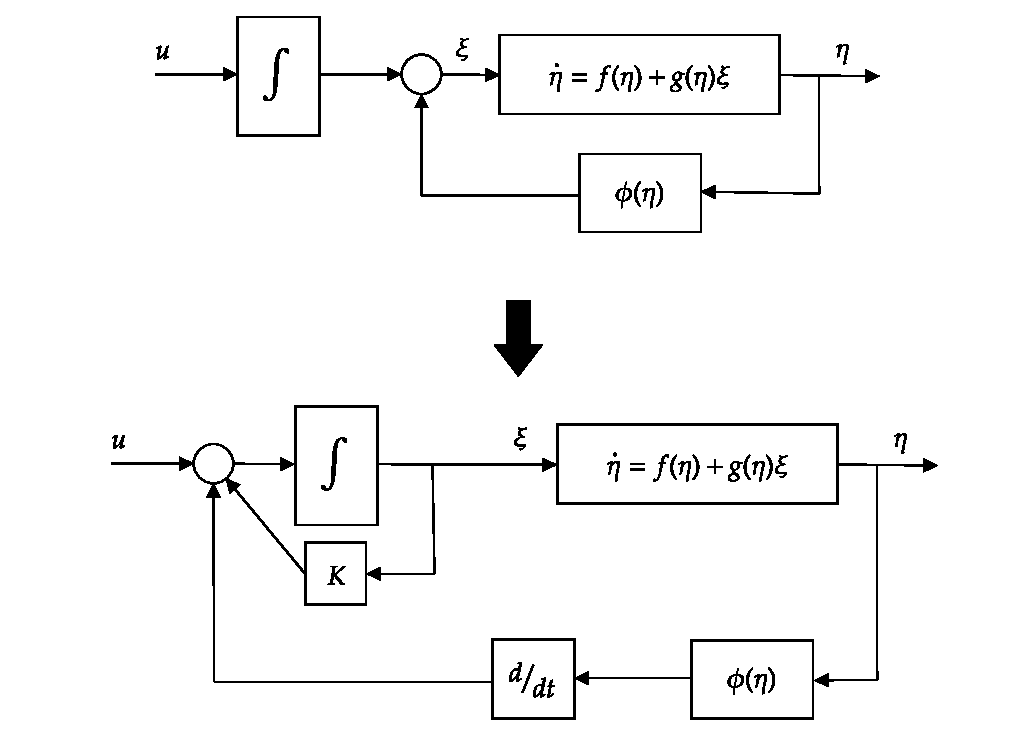
\includegraphics[width=0.8\textwidth]{img/backstepping_BlockDiagram.pdf}
	\caption{Idea básica del Backstepping de integrador.}
	\label{fig: backstepping_bloques}
\end{figure}

\subsection{Diseño del control virtual}
Véase a $\xi$ como una entrada de control virtual del sistema
\begin{equation}
	\dot{\eta} = f(\eta) + g(\eta)\xi.
	\label{eq: backstepping_esclavo}
\end{equation}
Suponga que existe una ley de control retroalimentado
\begin{equation*}
	\xi = \phi(\eta)
\end{equation*}
que estabiliza el origen de
\begin{equation*}
	\dot{\eta} = f(\eta) + g(\eta)\phi(\eta).
\end{equation*}
y que, además, conocemos una \gls{fl} $V(\eta)$ que lo asegura:

\begin{equation*}
	\dot{V}(\eta) = \dfrac{\partial(\eta)}{\partial \eta} [f(\eta) + g(\eta)\phi(\eta)] \leq -W(\eta), \quad \forall \eta \in D.
\end{equation*}

\subsection{Diseño del control verdadero por Backstepping}
\textbf{Cambio de coordenadas:} Como no se puede implementar el control virtual $\xi = \phi(\eta)$, definimos el error como una nueva variable
\begin{equation*}
	z = \xi - \phi(\eta).
\end{equation*}
Escribiendo el sistema en términos de esta nueva variable se obtiene
\begin{equation*}
	\begin{aligned}
		\dot{\eta} & = [f(\eta) + g(\eta)\phi(\eta)] + g(\eta)z,                                                         \\
		\dot{z}    & = u - \frac{\partial \phi(\eta)}{\partial \eta} [f(\eta) + g(\eta)\xi], \quad \xi = z + \phi(\eta).
	\end{aligned}
\end{equation*}
Si se diseña la variable de control como
\begin{equation*}
	u = -\dfrac{\partial \phi(\eta)}{\partial \eta} [f(\eta) + g(\eta)\xi] + v
\end{equation*}
entonces el sistema se describe como
\begin{equation}
	\begin{aligned}
		\dot{\eta} & = [f(\eta) + g(\eta)\phi(\eta)] + g(\eta)z, \\
		\dot{z}    & = v.
	\end{aligned}
	\label{eq: backstepping_z}
\end{equation}
\rmkb{
	¿Cuál es la diferencia entre \eqref{eq: backstepping_esclavo} y \eqref{eq: backstepping_z}? La diferencia es que en \eqref{eq: backstepping_z} el esclavo con la entrada proveniente del maestro igualada a cero $(z=0)$ tiene un \gls{pe} que es asintóticamente estable, esto es, el sistema es de Fase Mínima.\\

	En resumen, con un simple cambio de variables estabilizamos la \gls{dc} del sistema.\\

	Bastaría con estabilizar al maestro (que ya es lineal) y entonces el sistema completo tiene un \gls{pe} asintóticamente estable localmente (usando las ideas de linealización parcial).
}
La diferencia ahora, sin tomar el camino de Linealización Parcial, será construir una \gls{flc} para el sistema \eqref{eq: backstepping_z}, luego vamos a usar esa \gls{flc} para estabilizar al sistema completo \eqref{eq: backstepping_integrador}.

\subsubsection{Diseño del control por Lyapunov} El diseño se realiza proponiendo una \textbf{función candidata de Lyapunov}, en nuestro caso se puede usar
\begin{equation*}
	V_c(\eta, \xi) = V(\eta) + \dfrac{1}{2}z^2.
\end{equation*}
El control $v$ se elige de tal forma que $\dot{V}_c$:
\begin{equation*}
	\dot{V}_c = \underbrace{\dfrac{\partial V}{\partial \eta} [f(\eta) + g(\eta)\phi(\eta)]}_{<0} + \underbrace{\dfrac{\partial V(\eta)}{\partial \eta}g(\eta)z + zv}_{\text{diseñe } v}.
\end{equation*}
sea negativa definida. Aquí se propone
\begin{equation*}
	v = -\dfrac{\partial V(\eta)}{\partial \eta}g(\eta)z - kz, \quad k > 0.
\end{equation*}
con lo que
\begin{equation*}
	\dot{V}_c \leq -W(\eta) -kz^2,
\end{equation*}
donde
\begin{equation*}
	W(\eta) = \dfrac{\partial V(\eta)}{\partial \eta}g(\eta)z^2 - \dfrac{\partial V(\eta)}{\partial \eta}g(\eta)z.
\end{equation*}
El control $u$ finalmente, resulta ser
\begin{equation*}
	u = -\dfrac{\partial \phi(\eta)}{\partial \eta} [f(\eta) + g(\eta)\xi] - \dfrac{\partial V(\eta)}{\partial \eta}g(\eta)z - k(z + \phi(\eta)), \quad k > 0.
\end{equation*}
\rmkb{
	Note las siguientes diferencias importantes con respecto a la Linealización Parcial:
	\begin{itemize}
		\item La suma de las funciones de Lyapunov para los sistemas individuales se convierte en una función de Lyapunov para el sistema completo. Esto es gracias a la acción de control.

		\item El subsistema esclavo de la cascada no tiene que ser estable con entrada cero, sino que se puede estabilizar mediante el control virtual.
	\end{itemize}
}



